\chapter{Conceptual design}
\label{chap:conceptual_design}
This chapter is contains a discussion on the design of the different aspects of the requirement-to-test methodology. The discussion is started by defining an appropriate view on use case and then presenting three conceptual solutions along with a discussion on their applicability in the problem domain.\\\\
The goal is identify a suitable concept for a tool that enables us to inject better domain-awareness in our tests, and supports tests generation from them.
The concept should be designed to support loose structure, but still provide enough information test generation and basic requirement analysis.
% The constraint for not going after the optimum is added meta-model complexity.\\\\
\begin{figure}[!htbp]
\centering

\begin{tikzpicture}

% horizontal axis
\draw[->] (0,0) -- (6,0) node[anchor=north,midway] {\small Automation};

% vertical axis
\draw[->] (0,0) -- (0,4) node[anchor=south,rotate=90,midway] {\small Domain-awareness};

\draw (5,0.2) node[circle,fill,inner sep=1pt, fill=blue, label=above:1st iteration] {};

\draw (1.2,3.0) node[circle,fill,inner sep=1pt, fill=blue, label=above:2nd iteration] {};

% Project
\draw (5,3) node[circle,fill,inner sep=1pt, fill=dkgreen, minimum size=0.3cm, label=above:Project] {}; 

\end{tikzpicture}
\caption{Finding a good trade-off between domain-awareness and automation}
\label{fig:project_parameter_plot_project}
\end{figure}By discussing a iterating through a number of different conceptual designs, levering their benefits and disadvantages, a suitable model will hopefully emerge.

\section{Interpreting use cases}
While formalized use case models exist\cite{klimek2010formal}, they mostly focus on model checking and semantics. While this is indeed in important field of study, our scope is a bit different. As the tool we want to build here is meant as a support for existing development procedure -- rather than replacing it, and introducing formalism -- we constrain ourselves from constructing it from a formal model.\\\\
Instead we focus on the minimal structure, and build our way up from there. But, before we try to build up a model for use case that support test translation, we need to establish a common ground of what a use case is, what it should include, and what it shouldn't include. From \cite{cockburn2000} we get;
\begin{quote}
``... The use case, as the contract for behavior, captures \emph{all and only} the behaviors related to satisfy the stakeholders’ interests.''
\end{quote}which basically means that we should write our use cases, solely focusing on behavior and intent of the involved stakeholders. Any non-essential information should be left out. Another point that is commonly stated is that use cases should not be used to describe user interface actions, so for example an action ``user presses submit button'' is not suitable writing level for a use case.\\\\
So, in essence; use cases expresses \emph{expected system behavior from a stakeholder's point of view}. For this thesis we use the ``fully dressed'' use case template\cite{larman2005}, as it already provides very good structure to build upon. It specifies the need to include a stakeholder list, a primary actor, main scenario, pre- and postconditions and a list of extension that are linked to main scenario.
%IN SUMMARY; How much information can you acutally derive from a use case?

This section tries to extracts an abstract interpretation of a use case through a brief study of two use cases. The goal is to come up with a meta-model of use cases that captures the essentials of the informally written use case, and allow us to map the concepts from it to an abstract syntax so that test code may be generated from it.

The first use case is a basic phone call forwarding session that goes though a receptionist. The use case is described from the receptionist's point of view, as this is the scope of the main case study system. The use case has a detailed description that can be seen in appendix \ref{appendix:use-cases}. \\\\
The second use case is, in a sense, embedded in the first one as it part of the extensions of that use case. This will be covered later on. The use case covers a ``send message'' session typically done by having the receptionist actor transcribe a spoken message along with caller information (name, company, ...) onto a set of text input fields that then can be assembled to a message. This message is then handed over to the system that may enqueued it for later delivery -- or send it immediately, depending on implementation.


\section{Requirement-to-test process}
%Definition dictionary
% Remember that an actor has a set of goals, which he/she wants to realize through the system. Actor can be  primary (typically people) or supporting (provides service or information) - passive.
% A good goal has a verb/noun combination.
%REMEMBER TO TAKE INTO ACCOUNT <INCLUDE> use cases -- Basically extensions
Given the loose structure of the use case concept, we believe it is sufficient to treat preconditions as simply other use cases. A more elaborate motivation for this can be found in section \ref{sec:test_case_state}.\\\\
Postconditions can be defined to be predicates



Use case model terminology.
\begin{description}
  \item[Use case:]
  \item[Scenario:]
  \item[Entries:] Every step in the main scenario is composed of a entry. The entry may be decomposed into smaller components or just be a text, based on which level of detail we want. 
  \item[Extensions:]
  \item[Preconditions:]
  \item[Postconditions:]  
  \item[Domain actors:]
  \item[Domain concepts:]
\end{description}

Identified constraint in regards to test generation.
\begin{description}
  \item[Entries:] Every entry in a use case scenario is modeled as a synchronous self-contained action.
  \item[Termination:] A use case scenario should always terminate.
\end{description}

\section{Concept 1 - Markdown editor}
One of the earliest concepts for a tool to aid use case structuring, was an editor that used a markup language that enabled the user to tag specific words as keywords using a special syntax -- such as surrounding text with parentheses, or other significant characters. The concept was dropped in an early state, but is documented for completeness, and to reference some of the ideas introduced by it later on.\\\\
\begin{figure}[!htbp]
  \centering
  \includegraphics[width=0.70\textwidth]{\imgdir markdown_ui_mockup}
  \caption{Crude mock-up of a user interface using a markup language for writing use cases.}
\label{fig:markdown_ui_mockup}
\end{figure}The benefit that was hoped to gain from this procedure was that both the use case, and the extra data needed to generate tests, was stored in the same textual representation.\\
This concept was only implemented as an experimental prototype model without user interface, and proved too loose in structure to be able to implement within the time frame of this Thesis. The main problem was that it effectively required a domain-specific language to be able to support the structure needed for test generation. The creation of a domain-specific language was considered out of scope, and a too large task that would dominate the project, taking focus from the actual task.\\\\
Figure \ref{fig:markdown_ui_mockup} crudely shows how the user interface was planned to look like. Left part of the UI shows a structured textual representation of a use case. The middle part was reserved for graphical representations of the use case, which could be sequence diagrams or activity diagrams, and the right panel is for ``use case analysis'', which is associations that will become evident during a use case analysis. For example, ``user sends email'' implicitly states an association between ``user'' and ``email'. The tool was meant a online Wiki-like tool that enabled collaboration. The concept of markup language was dropped, but the concept of clear-text analysis was re-introduced later on.


\section{Concept 2 - Component/structure editor}
%TODO add some stuff about the fact that the concept was acutally implemented in a form of prototype.
This section presents the second requirement-to-test translation concept, proposes a rudimentary meta model and evaluates the approach in terms which parts should be refined in a later concept, and which shouldn't.
The second concept originated from the idea that structure could be added by a component-oriented tool. The user interface only provides graphical components that represent domain actors and concepts than can be connected and re-arranged to create the use cases. The user interface should then -- similar to the first concept -- provide immediate visual feedback in the form of textual use case representation (or a diagram), like in the first concept.\medskip

\noindent The procedure of the concept is to define actors and concepts beforehand, and then create use cases from combining these. So, if starting from scratch, a user would be expected to initially define at least one actor and the actions that the actor perform and the objects that this action would be performed on. This should be done prior to actually writing the use case.\medskip
\begin{figure}[!htbp]
\includegraphics[scale=0.4]{\imgdir test_case_ui}
\centering
\caption{Use case editor UI mockup}
\label{fig:use_case_editor_mockup}
\end{figure}

\noindent A user interface mock-up is shown in figure \ref{fig:use_case_editor_mockup}. In the top of the screen is a tab selector that selected the use case currently being edited. In the selected use case panel, we can see the main scenario (the selected tab), where the list use case steps are shown. The selected step is ``Receptionist send Message'', which is also shown in the bottom of the user interface, where it can be edited. The available actors and concepts are shown on the right side of the user interface. The pre- and postconditions are not included in the user interface mock-up, but are included in the meta model discussion.\medskip

\noindent The component/structure concept had the big advantage, that it was a good fit for -- and aided the development of -- the meta model. This concept was not chosen, due to the significantly increased workload that it involved, and the added meta model complexity. This is elaborated in the summary. The concept and its corresponding meta model was ultimately simplified for the next concept.

\subsection{Meta model}
This section contains a brief discussion of a meta model that could be used for translating use cases into test cases in this concept. The discussion is supported by the high-level graphical model depicted in figure \ref{fig:concept2_use_case_meta_model}, which shows the concepts that are being discussed.\medskip

\begin{figure}[h]
  \centering
  \includegraphics[scale=0.72]{\imgdir concept2_use_case_meta_model}
  \caption{Partial meta model for creating use cases models in concept 2}
  \label{fig:concept2_use_case_meta_model}
\end{figure}

\noindent The central class of the meta model is the use case. It is composed of stakeholders and a primary actor, pre- and post-conditions, use case steps (the \texttt{Step} class) and a number of extensions. The primary actor is mostly for information purposes, as the Actor class (which models the domain actor) is also contained within the steps. The \texttt{Step} class models the use case's steps, and are not very flexible as they expect a use case step to consist of an actor, a target and an action. The target may be either a domain actor or a domain concept.\medskip

\noindent The extensions are treated as lists of use case steps, as well as the main scenario. In addition, they have extension points, as well as optional return points to use cases. These map to the formulations where an actor returns to a specific step in the main scenario -- for example ``user returns to 2.'' -- in extensions. The pre- and postconditions are modeled as predicate classes, that ensures that some property holds for an associated concept.

\subsection{Mapping to application domain}
%GDR
In order to map the models produced with the tool, we need to translate them to models usable by the ``test mapping domain''. Figure \ref{fig:concept2_use_case_mapping} shows the conceptual model of how a meta model supporting this domain could look like. The discussion in this section will not go into too much depth with the meta model, as it has not been chosen as the implementation model. There may also be inaccuracies in it, for that exact reason.
\begin{figure}[!htbp]
  \centering
  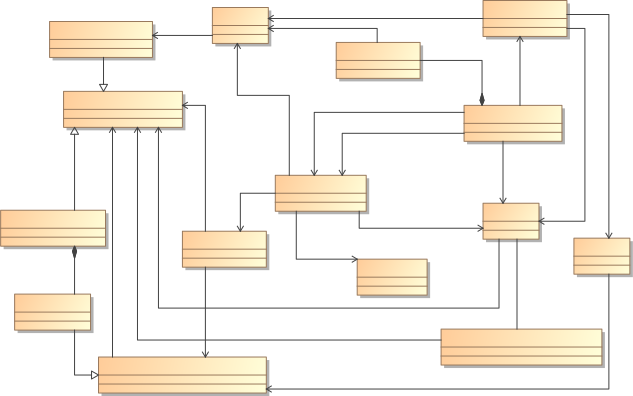
\includegraphics[scale=0.72]{img/concept2_use_case_mapping}
  \caption{Concept 2 use case mapping}
  \label{fig:concept2_use_case_mapping}
\end{figure}It specifies, like the meta model in figure \ref{fig:concept2_use_case_meta_model}, that the use case consists of an ordered list of steps, where actions consist of; one or more actors, one verb describing the action and one target for the action (object for verb). It also contains the corresponding associations to predicates (pre- and postconditions) and actors. But, unlike the simpler model for building the use case models, it is extended with additional classes, needed to construct models suitable for test generation. The mapping process is expected to be done by a developer, and could be realized by a textual test mapping language, discussed later in this section.\medskip

\noindent In the application domain, we have a set of domain actor, and domain concepts. The actors from the use case domain may be mapped to domain actors, acting in a specific role. In our system -- for example -- a ``contact'' actor may act as the ``callee'' in some use cases, which effectively is a role. A domain actor needs to be specialized by application domain actor classes, that need to be mostly coded by hand, but could be stubbed out by the tool. The wrapper class has the purpose of covering the domain concepts, functionality-wise. It will supply a set of methods, available for the developer to map to use case actions -- hence the association to the action class.\medskip

\noindent 
Predicates are treated as functional expressions, that link to a matcher which must be realized (in code) by a function that returns a boolean value, based on input. For instance, quantifications such as ``greater than'' and ``equals'' are examples of matchers.\medskip

\noindent 
One thing that proved useful, was the parameters of the test class. Basically, to be able to specify which domain concepts should be part of the signature of the test function. An example would be that a test function involving a receptionist actor, would need to have the signature \texttt{exampleTest(Receptionist r)}, or similar. The basic is just that the involved concepts, need to be supplied to the test function from the test support framework.
\subsection{Mapping language}
%TODO add something about how generated tests could look like.
In order to define the mappings from the use cases to the concepts in the meta model, the concept of a mapping language emerged. While the language never left the conceptual state, it is described in this section for completeness.\medskip

\noindent The mapping language is written in the aspect of an actor. It is conceptually the same as a recipe for a holder-class (class as i object-oriented programming) that knows about every interface that it needs to access, and every resource that needs to be provided to it.\medskip

\noindent The example language shown in figure \ref{lst:mapping_language_concept} illustrates how a language like that could look like. The example uses indentions to indicate ownerships. The label \textbf{Receptionist:} indicates that the mappings and properties below are owned by that actor. The requirements -- which could translate to class fields -- are listed (new-line separated) below the \textbf{requires:} keyword. The \textbf{maps:} keyword translates to provided methods (as those from the figure \ref{fig:concept2_use_case_mapping}). The methods have a signature, and a function body that should translate into a class method with the supplied body. These mappings are meant to be done, manually, by a developer (a mapper actor) trained in the method beforehand.\medskip

\begin{lstlisting}[caption=Example language for mapping concepts,label={lst:mapping_language_concept}]:
Receptionist:
  requires:
    MessageContentGenerator messageContentGenerator
    ReceptionistState currentState = ReceptionistState.Unknown
  
  provides:
    changeState (ReceptionistState rs) -> currentState = rs
  
  maps:
    sends_message (Message msg) -> msg.enqueue()

    types_in (Message msg) -> 
      msg.content = messageContentGenerator.next().content
    
    returns_to (ReceptionistState newState) -> this.changeState (newState)

  properties:
    is_ready -> receptionistState == ready
\end{lstlisting}

\subsection{Summary}
The concept outlined in this section was implemented on a prototype-basis -- without the mapping language or a user interface. The concept quickly proved infeasible for several reasons.
\begin{itemize}
  \item In order to create a use case, you first had to define every component (actor, action, concept) of the use case. This work-flow is quite cumbersome, and increases the work-load of creating use cases significantly. Having to decompose the use case before actually writing it is not very user friendly and shifts the focus from use case writing, to \emph{ad hoc} modeling.
  
  \item A potential problem with this approach is that the rigid structure of having the actor-action-object constraint could quickly lead to artificial use cases that fitted the tool, rather than the problem domain. As it would be very close to the implementation, it was also speculated that terms from it would find its way back into the requirements. This would lead to a too technical jargon in use cases. This is generally a bad idea as it alienates the customer \cite{christel1992}.

  \item The predicates provided little, or no value in the experimental prototype that was implemented, and revealed that they could be written in the mapping code very easily without the need to include them in the meta model.

  \item The problem with the mapping language is, that it came very close to a programming class, and it felt very much like re-inventing object-oriented programming classes. The very big benefit of having a mapping language, was that the meta model of a system under test could be linked to that of our use cases, and provide a much better analysis of the use case translation. It would, thus, enable tool-level analysis awareness of missing mappings.

\end{itemize}
There were some good concepts that proved useful in the next concept. Mainly, the idea of inferring knowledge about \emph{who} (domain actors) is performing an action and \emph{what} (domain concepts) is the target for the action. This is very useful information when we need to extract information about what the resource requirements for the tests should be. The idea of pre-defining some of the concepts and actors for the use cases to share is also carried on to the next concept.


\section{Concept 3 - Hinting tool}
\label{sec:3rd-iteration}
\begin{figure}[!htbp]
  \centering
  \subbottom[Actors tab\label{sfig:customer-ui-mockup-actors}]{%
    \includegraphics[width=0.49\linewidth]{\imgdir customer-ui-mockup-actors}}
  \subbottom[Uses cases tab\label{sfig:customer-ui-mockup-use-cases}]{%
    \includegraphics[width=0.49\linewidth]{\imgdir customer-ui-mockup-use-cases}}
    
  \subbottom[Definitions tab\label{sfig:customer-ui-mockup-definitions}]{%
    \includegraphics[width=0.49\linewidth]{\imgdir customer-ui-mockup-definitions}}
  \caption{Mock-up screens of the customer user interface.}
  \label{fig:concept3-mockup-screens}
\end{figure}
\noindent The third concept is a hybrid between the first second concept introduced in this chapter. It is place -- functionality-wise -- somewhere in between. It kept the ability to predefine actors and concepts, but didn't enforce the composition structure as the previous concept. The use cases were kept as text-only steps that could be analyzed using the defined actors and concept at any point -- after they are written. The basics of the concept is ``type hinting'' or ``visually annotating'', as it will derive actor types an concepts from the use cases, using text-matching. From these type hints, the tool would then be able know which resources should be provided to tests in the test generation step. The concept is implemented as the current prototype.\medskip

\noindent Figure \ref{fig:concept3-mockup-screens} outline the screens expected in a user interface of realizing this concept. The first tab of mock-up -- depicted in figure \ref{sfig:customer-ui-mockup-actors} -- show an overview of the actors defined. Currently, only the ``User'' actor is defined, and this actor has some associations and capabilities, that are extracted from the definitions created, and use cases that the user partakes in. The next tab, which is depicted in figure \ref{sfig:customer-ui-mockup-use-cases}, show the selected use case with the different parts highlighted. One color for actors, one for actions, one for objects. Figure \ref{sfig:customer-ui-mockup-definitions} show a tab that contains the current definitions. A \textbf{definition} is the representation of meta-model concept (or actor) in a particular role. This definition needs a unique name, which should correspond to a concept already found in the domain model. The domain model, if defined beforehand, could also be thought to be a imported to the declarations.

\subsection{Hinting process}
The purpose of this section is explain of the hinting process through an example. The section starts from a use case description, and tries to go through the steps needed to convert it into an acceptance tests. The use case used in this text is simplified and contain only the basics needed for interpreting and translating the use case. It is shown in verbatim text seen in listing \ref{lst:uc-simple-example}, and does not illustrate any user interface specific details. It contains three lists; the main scenario, the postconditions and the preconditions. Each of these lists are simple text strings.

\begin{lstlisting}[frame=single,style=usecase, caption=Use case example, label=lst:uc-simple-example]
Scenario:
  Receptionist types in message
  Receptionist sends message
  Receptionist marks state as ready 
Preconditions:
  The receptionist is logged in
Postconditions:
  The message is stored
  The receptionist is ready to handle the next call
\end{lstlisting}
The first thing we need to do to translate this example, is that we identify the domain concept contained within the list steps in the text. In this case, we here observe that it includes the concept ``message'' a ``receptionist'' actor. additionally; some interaction between the message and the actor, which we define as actions.\medskip

\noindent In listing \ref{lst:uc-simple-example-highlighted} we have highlighted the different parts of the use case, using an orange color for actors, green for actions, blue for domain concepts, and a dark red for attributes. Using this highlight, it illustrates the abstract interpretation and the interaction between the different part very well. In this case, the actor role names match their domain actor names, but it is important to note that the participating actors (and concepts), participate in a role -- rather than as an actor. The role of definitions are also illustrated in the domain model later on.
\begin{lstlisting}[frame=single,style=usecase, caption=Use case example with its different parts highlighted, label=lst:uc-simple-example-highlighted]
Scenario:
  @\color{orange} Receptionist@ @\color{dkgreen}{types in}@ @\color{blue}{message}@
  @\color{orange} Receptionist@ @\color{dkgreen}{sends}@ @\color{blue}message@
  @\color{orange} Receptionist@ @\color{dkgreen}{marks state}@ as @\color{blue}{ready}@
Preconditions:
  The @\color{orange}receptionist@ is @\color{dkred}logged in@
Postconditions:
  The @\color{blue}message@ @\color{dkred}is stored@
  The @\color{orange}receptionist@ @\color{dkred}is ready@ to handle the next call
\end{lstlisting} 
Based upon the information in listing \ref{lst:uc-simple-example-highlighted}, we extract the components from the use case and translate it into test code that could look like listing \ref{lst:uc2_example_test_code}. In the tests, each of the concepts in the example is mapped to a class, that is given an object identifier. In this case, we have the ``Receptionist'' and ``Message'' classes that have the identifiers ``receptionist'' and ``message'' -- respectively.\medskip

\noindent Given the amount of information in (and definitions of) the use cases, we can easily generate code such as the one shown in listing \ref{lst:uc2_example_test_code}. But these functions are still very high-level, and doesn't assert anything about the system being tested, it's just an alternate representation of the use cases. To be able to actually test the implementation, we need to fill in the methods used on our receptionist and message object. The methods will act as the link between the tests and the implementation, which is the mappings. The mappings are -- in this conceptual model -- meant to be written manually by a developer. Most of the code can probably be generated as stubs. The next sections goes through the test function, discusses the individual parts in more detail, and suggests conceptual implementation mappings by classifying them.
\begin{lstlisting}[style=Dart, caption=Suggested structure of generated test case,label={lst:uc2_example_test_code}]
boolean usecase_test (Receptionist receptionist, Message message) {
  // Preconditions
  expect (receptionist.is_logged_in(), true);

  // Scenario
  receptionist.types_in (message);
  receptionist.sends (message);
  receptionist.marks_state (idle);
  
  // Postcondition
  expect (message.is_stored(), true);
  expect (receptionist.is_ready(), true);
}
\end{lstlisting}
Prior to running the test function, the supporting test tools (covered in \ref{ssec:supporting-test-tools}) needs to supply the objects ``message'' and ``receptionist'' pre-initialized. This makes them a very explicit part of the resource dependencies to the test, and should be added to the signature of the test function. The dependencies are extracted from the resources requirements of the test function block.\medskip

\noindent The second thing that needs to be done is to add the preconditions. Having tagged the types and the property of that must hold, we can translate the precondition into an ``expect'' expression.\medskip

\noindent Next of the test, the statement \texttt{receptionist.types\_in~(message)} is a method that belongs to the receptionist actor, and requires knowledge of the ``message'' domain concept. The action of typing in a message is conceptually the creation of message object. So, to be able to make meaning of the test, we need some way of simulating the message creation. This infers the need for a content generator mechanism. A concrete implementation could be a simply fixed ``dummy object'' or an object that is generated with content from a randomized pool. In the pseudo-code in listing \ref{lst:code_for_receptionist_domain_actor} a MessageContentGenerator is associated with the Receptionist class as a basic class field.
\begin{lstlisting}[style=Dart, caption=Pseudo code representing Receptionist domain actor,label={lst:code_for_receptionist_domain_actor}]
class Receptionist {
   MessageContentGenerator messageContentGenerator= ...;
   ReceptionistState receptionistState = ...;
  
  void types_in (message) {
  	message.updateContent(messageContentGenerator.content);
  }
  
  void sends (Message message) {
    message.enqueue();
  }
  
  // Alias function.
  void returns_to (State newState) {
  	changeState (newState);
  }
  
  void changeState (State newState){
  	receptionistState = newState;
  }
  
  boolean is_ready() {
    return receptionistState == ready;
  }
}
\end{lstlisting}
The next statement in listing \ref{lst:uc2_example_test_code}; \texttt{receptionist.sends (message)} takes the argument ``message'' and makes it available for other actors to access later on, by storing it persistently. This is typically done using a database or file store. By sending a message to a message store, we can delegate the action to an ``enqueue'' method of the message object, which needs to have a notion of where it is, or should be stored. This is realized by having a ``messageStore'' interface which is a service interface object that, can actually be originating directly from the code base of the system under test.\medskip

\noindent The final statement in the scenario is \texttt{receptionist.returns\_to (ready\_state)}. This is actually a mutation function that alters the state of the receptionist actor. This state change could be global and should then  be updated multiple places, which then leads to additional ``state-store'' dependencies. Here, we also note that there is a concept of a ready\_state this is an explicit state change that could, possibly be linked to a state machine (see \ref{ssec:target-system-state} contained within the receptionist actor object.\medskip

\noindent The final thing done in the tests, is the postconditions, which are translated to expressions corresponding to preconditions.\medskip

\noindent An open question that was raised during the development of this concept is; how much extra information can we add. Can we use some extra classifiers to increase the test generators understanding of the annotated use cases? For example; if we were to add a ``persistent concept'' annotation to message, would it improve test generation?\medskip

\noindent The pseudo code for the ``Message'' class is shown in listing \ref{lst:code_for_domain_concept} for completeness, and will not be discussed in detail.
\begin{lstlisting}[style=Dart, caption=Pseudo code representing Message domain concept,label={lst:code_for_domain_concept}]
class Message {
  RESTMessageClient messageStore = ...;
  
  void enqueue() {
    messageStore.enqueue(message);
  }

  boolean message.is_stored() {
    messageStore.contains(this);
  }
}
\end{lstlisting}
\subsection{Evaluation}
There is a lot of manual work associated with this process, as the only help you will receive from the conversion tools, are method stubs. This, however provides programmers with good guidelines on what the method should do. The lowered value compared to the second concept is, that we no longer have a complete view -- from the use case tool -- of the test model. On the other hand, in this concept, developers can write the tests using a general purpose language that they should be more comfortable with, rather than a mapping which must be learned first.\medskip

\noindent This concept is -- as previously mentioned -- implemented in the current prototype of the tool. The form is, however not identical to the concept introduced here, but simplified further, which we shall also see in the next chapter.\medskip

\noindent A common denominator for all three concepts, is that manual mapping seems to be necessity. In the second concept, a mapping language was introduced, but the fact that it almost mirrored the concept of a programming class, made it infeasible. In particular because developers, learning a new language is costly, and the gain from learning to use it did not match the questionable value of getting a mapping model.

\begin{figure}[ht]
\centering
\includegraphics[width=0.7\textwidth]{\imgdir event-stack-to-state-machine}
\caption{Concept; validate event stack using life-cycle state machines.}
\label{fig:event-stack-to-state-machine}
\end{figure}
%\section{Object tracking} NOTE: Maybe something about object lifecycles (and statemachines for them) here.

\begin{figure}[ht]
\centering
\begin{drawstack}
  % Within the environment, draw stack elements with \cell{...}
  \cell{lock}
  \cell{unlock}
\end{drawstack}
\caption{Event stack}
\label{fig:event-stack-example}
\end{figure}

Some basics on the procedure; take every line of the use case and not every concept and actor used. Then speculate on the realization of this. Which components should be involved, and which other actors. Depending on the concrete architecture, these components may be services, larger program components (such as Java packages), or even sub-functions.



%TODO Overall generation concept. A test needs to be supplied with some resources as input.